% --------------------------------------------------------------------



\section{Introduction}

In recent years the web service landscape has exploded 
with users and available services. Every aspect of our lives 
has been infiltrated by apps and web services to 
an extent that brick and mortar businesses are rapidly declining 
and have to reinvent them selves (VERIFYING light SOURCE!).
Finally the promises given in before the Dot Com bubble burst 
in the end of the 20th century have delivered.

The rapid expansion and at times as fast decline of web services 
need a matching architecture to meet these very specific needs. 
Monoliths have served us well but the time has come to evolve with the customer needs.

Microservice Architecture (MSA) differs in many ways from 
the more tradition Monolith Architecture (MA). This shift entails very specific security issues.

In this thesis the MSA and security literature is evaluated and the main differences between
MA and MSA security aspects are found.





\section{Definitions}

In this thesis the following definitions are used.

\subsection{Architecture}

TODO


\subsection{Microservice}

A microservice is a service that: is independently deployable,
is modeled around business domain,
that owns the data that they need to operate,
that communicates via network,
is technology agnostic,
that encapsulates data storage and retrieval and 
that has stable interface \citep{newman2019}.

\subsection{Monolith}

TODO

\subsection{Security}

Security can be defined in multiple ways but in this thesis security 
and more specifically information security is defined as consisting of 
Confidentiality, Integrity, and Availability (CIA) as is stated in the 
pocket book on ISO/IEC 27001 -standard for information security \citep{isoiec27001}.

The ISO/IEC 27001 standard defines confidentiality as such that information or property 
is available to the authorized user only.
Integrity means that the data or property is safeguarded for accuracy and completeness.
Availability in this web service context is defined as such that the property or information 
is only available or diclosed to authorized users.
The authorized users can consist of persons, processes or entities to whom 
the information or property can be disclosed.


\section{Random text}

Developing software using the MA the structure the whole application or service 
is usually deployed as a whole and the program code can be compiled, tested and
used as a single unit or multiple modules. In contrast to this a service implemented 
by using a MSA can be deployed in single microservice units and thus a single service 
can be worked upon individually.






% Kokeile mitä kappaleen viimeisen rivin lopulle käy, 
% kun sloppypar-ympäristön kommentoi pois: joku rivi
% saattaa ylittää marginaalin. Sloppypar-ympäristössä
% sanojen välissä olevaa tyhjää voi olla enemmänkin
% jotta marginaalin ylityksiä ei tapahdu.
\begin{sloppypar}

\end{sloppypar}

\subsection{Microservice}
% Sanni Heinzmann

%\textbf{TIK.kand kommentti: Helpota lukijan työtä kaikin
%mahdollisin tavoin. Haluat voittaa lukijan omalle puolellesi.
%Lukijalle on hyvä tuoda heti alusta selville, mihin pyrit.
%Verratuna kaunokirjallisuuteen: ``kerro heti kuka murhaaja on''}

% --------------------------------------------------------------------

% \section{Kandidaatintyön rakenne- ja muotoseikat}
% \label{sec:esimluku}

% Tässä luvussa esitellään kandidaatintyön muotovaatimuksia
% tällä kurssilla. Muutamat alkuperäiset lähteet ovat saattaneet
% kadota organisaatio- ja tietojärjestelmämuutoksissa, kun
% Into-järjestelmä on korvannut WWW-sivustoja.

% \subsection{TKK:n kandidaattityöryhmän ohjeistus}

% Yleiset kandidaatintyön muotovaatimukset on annettu TKK:n
% kandidaattityöryhmän päätöksellä 14.11.2006 ja ne ovat
% kokonaisuudessaan saatavissa osoitteessa
% \url{http://www.tkk.fi/fi/opinnot/opintohallinto/paatokset/kandi20061114.pdf}.
% Tässä luvussa annetaan lyhyt, selvennetty ja joiltakin osiltaan
% karsittu yhteenveto kyseisistä ohjeista. Seuraavassa viitataan siis
% edellä mainittuihin TKK:n kandidaatintyön ohjeisiin (esim. ``luku 3''
% tarkoittaa TKK:n kandidaatintyön ohjeiden lukua kolme).

% \textbf{TIK.kand suositus: Lue alkuperäiset ohjeet erityisesti
%   silloin, jos et kirjoita työtä annettua \LaTeX{}-pohjaa käyttäen.}

% TKK:n kandidaatintyön ohjeissa käsitellään työn rakennetta (luvussa 3)
% ja muotoseikkoja (luvussa 4). Yleisesti todetaan kandidaatintyöstä
% seuraavaa:
% %
% \begin{quotation}
% \noindent \it
% Kandidaatintyö voi perustua teoreettisen taustan tarkasteluun 
% ja sen analysointiin sekä johtopäätösten tekoon tai kokeelliseen osioon ja 
% tulosten analysointiin sekä johtopäätösten tekoon
% tai edellisten yhdistelmään.
% Kandidaatintyön rakenteen tulee olla hyvän tieteellisen kirjoittamisen 
% käytännön mukainen
% ja sisältävän vähintään seuraavat osat: [$\ldots$] (Luku 3)
% \end{quotation}

% Rakenteen osia ovat: nimiölehti, tiivistelmä, sisällysluettelo,
% symboli- ja lyhenneluettelo (työn luonteen vaatiessa voi puuttua),
% johdanto, aikaisempi tutkimus (työn luonteen vaatiessa teoreettinen
% tausta), tutkimusongelma ja -menetelmät, tulokset, tarkastelu (työn
% luonteen vaatiessa johtopäätökset tai näiden yhdistelmä), lähteet,
% liitteet (jos tarpeen). Osat johdannosta tarkasteluun muodostavan työn
% tekstiosan. (Luku 3) Tekstiosan sopiva pituus on 15--20 sivua eikä
% työtä ole syytä tarpeettomasti pidentää (luku 4.2.1).
% Kokonaissivumäärä tulee tällöin olemaan noin 18--25 sivua.

% Muotoseikoissa TKK:n kandidaatintyön ohjeissa otetaan esille, että
% työn tulee olla jäsennelty ja tyylillisesti sekä kielellisesti
% viimeistelty ja moitteeton.  Tarpeettomia tyylillisiä erikoisuuksia
% tulee välttää.  Tekstiosassa tulee olla vain työn kannalta oleelliset
% kuvat tai taulukot. (Luku 4.1)
% %
% Kirjasinlaji tulee olla roomalaistyyppinen (Times New Roman
% tai Computer Modern\footnote{\LaTeX{}in perusfontti}) ja kooltaan 12 pistettä
% (luku 4.2.2). 
% %
% Työn nimessä ei saa esiintyä lyhenteitä, kaavoja tai lainauksia
% (luku 4.2.3).

% Nimiölehdellä tulee olla tiedot yliopistosta, tutkinto-ohjelmasta,
% työn nimestä, luonteesta (``Kandidaatintyö''), päivämäärä ja tekijän
% nimi (luku 4.2.4). Tiivistelmäsivusta esitetään vastaavat seikat,
% jotka löytyvät myös tarjolla olevista pohjista
% (doc\footnote{\url{http://peppi.hut.fi/pub/kandi/kandi.php}} tai tämä
% \LaTeX{}-pohja).  Se ei saa olla sivua pidempi. 
% % WANHA:
% %Tiivistelmässä
% %ilmoitettavaan sivumäärään lasketaan tekstiosan lisäksi
% %lähdeluetteloon kuluvat sivut. (Luku 4.2.5)
% Tiivistelmässä
% ilmoitettavaan sivumäärään lasketaan kaikki sivut yhteen 
% nimiölehdestä lähdeluettelon tai liitteiden loppuun
% (Kirjaston suullinen ohje 29.8.2011). 

% Asemoinnin suhteen tekstiosaa ei sisennetä vaan kappaleiden väliin
% jätetään yksi tyhjä rivi. Jos oikea reuna tasataan, niin tulee käyttää
% tavutusta ja tarkistaa, että se menee oikein.  Rivivälin tulee olla 1
% tai 1,5. (Luku 2.4.7)

% Huomaa, että TKK:n kandidaatintyön ohjeissa sivujen numeroinnin ohjeet
% ovat ristiriitaiset (luku 4.2.6). Oikea sivunumeroinnin malli on
% toteutettu tässä pohjassa.  

% Lähdeviittaukset tulee tehdä huolellisesti ja samanmuotoisesti joko
% nimi-vuosi- tai numerojärjestelmällä. Alaviitejärjestelmää ei
% suositella. (Luku 2.4.8)

% \textbf{TIK.kand suositus: Numerointi aloitetaan arabialaisilla
%   numeroilla nimiölehdestä kuitenkin niin, ettei numeroa kirjoiteta
%   sille. Siten ensimmäisen tiivistelmäsivun sivunumero on 2. 
%   Kirjasinkoko on 12, riviväli 1,5. Tekstiviitteissä käytetään
%   nimi-vuosi-järjestelmää, mutta tässä ohjaajan sana on määräävä.}

% \subsection{TIK.kand: kommentteja rakenne- ja muotoseikoista}

% Tekstiasun viimeistelyyn tulee varata runsaasti aikaa V3- ja
% V4-palautusten väliin. Työn tulisi olla oleellisesti valmis jo
% V3-palautuksessa, jotta ohjaajasi voi antaa palautetta, kuinka työ
% viimeistellään ja saadaan hyväksi kokonaisuudeksi, ja sinulla on 
% tarpeeksi aikaa hienosäätöön.

% Huomaa, että sivumäärä on hyvin riippuvainen tekstin luonteesta:
% pelkkää tekstiä mahtuu tässä \LaTeX{}-pohjassa sivulle noin 300 sanaa,
% kun taas jos mukana on kuvia, luetteloita tai paljon väliotsikkoja,
% sanamäärä on huomattavasti pienempi. Vastaavasti pienempi riviväli tai
% fonttikoko antaa lisää sanoja sivua kohden.

% Luennolla 6.9.2011 kurssin vastuuopettaja Tomi Janhunen linjasi, että
% sivumäärä ei ole kriittisin asia vaan itse aiheen käsittely.  Jos
% sivumäärä poikkeaa, ohjaaja tai kurssin henkilökunta voi puuttua
% tilanteeseen. Jos sivumäärä on pieni, voidaan kysyä, onko aihetta
% käsitelty tarpeeksi laajasti tai onko selittämiseen tai perusteluihin
% käytetty vaivaa. Toisaalta iso sivumäärä voi kertoa siitä, ettei työn
% rajaamista ole hallittu, ja tämäkin voi olla arviointiin liittyvä
% tekijä. Myöskään ei saa ajatella sitä, että kun 20 sivua tekstiä tulee
% täyteen, niin opinnäytetyö on valmis. Tieteellisen tekstin
% kirjoittaminen on iteratiivista: kirjoitetaan, luetaan, karsitaan ja
% lisätään, kirjoitetaan uudestaan, luetaan, jne. Tyypillisesti
% sivumäärän kanssa ei tule ongelmaa: annetusta tehtävästä tällä
% aikataululla tulee tyypillisesti noin 20 sivun mittainen raportti.

% Ohjeita kandidaatintyön eri osien kirjoittamiseen on sisällytetty
% tähän pohjaan. Kirjoittamisohjeita on koskien tiivistelmää, käytetyt
% lyhenteet -osiota, johdantoa, loppulukua ja liitteitä.  Lisäksi
% lähdekoodissa \verb!main.tex! on ohjeita alkusanoihin, joiden käyttöä
% ei suositella kandidaatintyössä.

% \subsection{Kirjallisuutta}

% Seuraavat kolme kirjaa löytyvät T-kirjaston käsikirjastosta:
% %
% \begin{itemize}
% \item \cite{kauranen2006} ovat kirjoittaneet kirjan erityisesti TKK:n
%   opinnäytetöitä ajatellen.  Kirjaa saa pääkirjastosta 8 euron
%   hintaan.
% %
% \item ``Tutki ja kirjoita'' \citep{hirsjarvi2009} lienee Suomessa alan
%   perusteos.  Kirjan hinta on noin 60--70 euroa.  T-talon kirjastossa
%   on kohdassa ``Yleistä 0'' muutamia vanhempia painoksia kirjasta.
% %
% \item Kielenhuollon opas \citep{oikeinkirjoitus2010} tarjoaa apua
%   oikeinkirjoitukseen. Kirjaa saa Kotimaisten kielten
%   tutkimuskeskuksen verkkokaupasta
%   \url{http://www.kotus.fi/index.phtml?s=2420} 20 euron hintaan.
% \end{itemize}

% Kurssiesitteeessä Nopassa on myös linkkejä lukuisiin 
% kotimaisiin Internet-sivustoihin opinnäytetyön kirjoittamisesta.
% Näitä ovat mm.
% %
% \begin{itemize}
% \item Oulun yliopiston ``Kirjoittamisen ABC''
%   \url{http://webcgi.oulu.fi/oykk/abc}
% %
% \item Helsingin yliopioston puhe- ja kirjoitusviestinnän opas
%   ``Kielijelppi'' \url{http://www.kielijelppi.fi/}
% %
% \item Oman kirjastomme tarjoama tiedonhaun itseopiskelupaketti
%   \url{http://peppi.hut.fi/pub/opetus/tiedonhaku/pmwiki.php}
% %
% \item Yucca Korpela on kirjoittanut nettioppaan ``Arkisen
%   asiakirjoittamisen opas'' \url{http://www.cs.tut.fi/~jkorpela/kirj/}
% \item Aalto-yliopiston Opiskelutaidot-sivusto \\
%   \url{https://into.aalto.fi/ display/ fiopiskelutaidot/}
% %
% \end{itemize}


% --------------------------------------------------------------------

% \section{Esimerkkejä \LaTeX{}in käytöstä}
% \label{sec:esimluku}

% Tässä luvussa annetaan esimerkkejä tyypillisimpiin
% kirjoitustehtäviin. Katso siis valmista PDF-tiedostoa ja lähdetekstiä
% tiedostossa \verb!luku_sisalto.tex!. Katso myös varsinaista
% päätiedostoa \verb!main.tex! ja etenkin sen alkua, jossa ladataan
% lisäpaketteja (sisältäen komentoja). Tämän dokumentin sivuasettelut
% tehdään pääosin tyylitiedostossa \verb!aaltosci_t.sty!, jota ei tulisi
% itse muuttaa lainkaan.

% Tarkempia ohjeita voi etsiä kirjallisuudesta tai Internetistä
% sopivilla hakusanoilla. Apua suomeksi: \citet{lyhyt2e},
% \citet{mattakivela}, Wikibooksin LaTeX-opas%
% \footnote{http://en.wikibooks.org/wiki/LaTeX/}, Jukka Korpelan
% LaTeX-sivut%
% \footnote{http://www.cs.tut.fi/~jkorpela/softa/latex.html} yms.
% Järkäleteoksia, mm.  \citet{mittelbach2004}, on saatavilla myös
% kirjaston sivujen kautta e-kirjana. Googlaamalla ``latex <ongelmasi
% avainsanoja>'' löytyy varmasti apua.

% \subsection{\LaTeX{}in asennus ja taustaa}
% \label{sec:esimlatexajo}

% TeX-jakeluita on saatavilla ``kaikkiin'' eri ympäristöihin.
% Suositeltavaa (helpointa?) on käyttää koulun omia Linux-ympäristöjä,
% jolloin tarvittavat tausta-asetukset lienevät kunnossa.  Windows- ja
% Mac-koneille on saatavana eri TeX-jakeluja, mm.
% TeXlipse\footnote{\url{http://texlipse.sourceforge.net/}} (Eclipsen
% liitännäinen) ja MiKTeX\footnote{\url{http://miktex.org/}}.

% \subsubsection{Lähdetiedostosta PDF:ksi}
% \label{sec:esimkaannos}

% Tässä zip-paketissa on mukana \verb!Makefile! (päivitä
% omat tex- ja bib-tiedostojen nimet), joten pelkkä komento
% \verb!make! riittää. Olkoon tässä päätiedoston nimi \verb!main.tex! --
% voit sen vaihtaa luonnollisesti miksi tahansa.

% Jos ajat \LaTeX{}ia komentoriviltä tai jostain graafisesta ikkunasta,
% niin ``käännä ja kaulitse'' \verb!pdflatex main.tex! tarvittaessa kaksikin
% kertaa. Kun olet lisännyt tekstiviitteitä komenna \verb!pdflatex main!,
% \verb!bibtex main!, \verb!pdflatex main!, \verb!pdflatex main!. Tarkkaile
% ruudulle tulevaa tulostusta; esimerkiksi:
% %
% \begin{verbatim}
% Package natbib Warning: Citation(s) may have changed.
% (natbib)                Rerun to get citations correct.
% \end{verbatim}

% Käännösvaiheissa hakemistoon ilmestyy monenlaisia työ- ja 
% lokitiedostoja, joiden päätteinä mm. aux, log, toc, bbl, blg.
% Joskus voi olla syytä poistaa nämä komentamalla \verb!make clean!.

% \subsubsection{Ongelmien ratkaisija: \LaTeX{} checker}
% \label{sec:esimlacheck}

% Sopiva tekstieditori (emacs, TeXLive, LEd, $\ldots$) osaa
% neuvoja, kun joku tekstissä on joku kielioppivirhe. Tämän 
% lisäksi oiva työkalu on \verb!lacheck!, joka löytyy (?)
% unix-koneista asennettuna ja ladattavissa 
% Windows-koneelle%
% \footnote{\url{http://www.ctan.org/tex-archive/support/lacheck/}}.
% Komennon \verb!lacheck main.tex! (\verb!lacheckw32 main.tex!)
% tulostuksesta voi helposti etsiä, missä kohtaa on jäänyt joku
% sulku tai ympäristö sulkematta kiinni. Alla olevassa listauksessa
% vika löytyy rivin 224 läheisyydestä.
% %
% \small
% \begin{verbatim}
% ** luku_sisalto:
% "luku_sisalto.tex", line 178: missing `\ ' after "engl."
% "luku_sisalto.tex", line 224: <- unmatched "\end{center}"
% "luku_sisalto.tex", line 1: -> unmatched "beginning of file luku_sisalto.tex"
% "luku_sisalto.tex", line 506: <- unmatched "end of file luku_sisalto.tex"
% "main.tex", line 48: -> unmatched "\begin{document}"
% \end{verbatim}
% \normalsize

% \subsubsection{``Ääkköset eivät ole enää ongelma''}

% Katso tiedoston \verb!main.tex! alkua. Näppäimistön merkistökoodaus
% valitaan kohdassa \verb!inputenc!. Kaikkien lähdetiedostojen tulee
% olla saman merkistökoodauksen mukaisia.  Useat editorit osaavat
% vaihtaa koodausta; pääosin on tarve vaihtaa ISO-8859-1 (Latin 1) ja
% UTF-8 (Unicode) välillä. Linuxissa voit katsoa tiedoston koodauksen
% \verb!file -i tiedosto.tex! ja muuttaa sen tarvittaessa\\
% \verb!iconv -f ISO_8859-1 -t UTF8 fileLatin1.tex > fileUTF8.tex!.

% Kohdassa \verb!fontenc! kerrotaan, millaista ulostuloa \verb!pdflatex!in
% halutaan antavan. Tämä näkyy esimerkiksi siinä, ovatko kirjaimet
% bittikarttoja vai vektorigrafiikkaa (suurenna PDF-selaimessa 1600\%)
% tai miten ääkköset esitetään (kopioi ja liitä tekstiä ruudulta 
% tekstieditoriin; näkyykö ä \verb!ä!:nä vai \verb!\"a!:na.

% Tämän zip-paketin tiedostot ovat UTF8-koodattuja.

% \subsubsection{Tavutus ei toimi?}
% \label{sec:esim_tavutus}

% \LaTeX{} osaa tavuttaa melko lailla oikein, kun valitaan \verb!babel!illa
% oikea kieli. Joidenkin hankalien sanojen osalta voit auttaa
% ehdottamalla tavurajoja paikallisesti \verb!ta\-vu\-ra\-ja!
% tai koko tekstin osalta \verb!\hyphenation{}!-määrittelyssä
% \verb!main.tex!:n alussa. Jos tavutus ei toimi, varmista merkistökoodaus
% (UTF-8 / ISO-8859-1). Varmista myös, että valittuna tekstissä oikea kieli
% komennolla \verb!\selectlanguage!.

% Testaa myös kääntöä IT-keskuksen koneissa -- jos
% toimii koululla, niin omasta jakelusta puuttuu \verb!babel!.
% Katso myös luvun~\ref{sec:hienos} \verb!sloppypar!-ympäristö.

% \subsubsection{Oikoluku}

% Oikoluvun suoran tuen puute on yksi iso ongelma kirjoitettaessa suomeksi.
% Yksi mahdollisuus on kopioida teksti johonkin oikolukijaan. Helpompi
% tapa lienee kopioida tiedostot Linux-koneille, joissa
% suomenkielisen tekstin voi oikolukea Voikkoa käyttäen tex-tiedostoista
% \verb!tmispell -dsuomi -t main.tex!.
% Ohjelman \verb!tmispell! vipu \verb!-t! jättää \LaTeX{}-komennot
% huomioimatta. Ohjelma saattaa lukea vain UTF8:aa, joten 
% tällöin tiedostot on muutettava tai kopioitava \verb!iconv!illa,
% katso ääkköslukua yllä.

% \subsubsection{Hienosäätö}
% \label{sec:hienos}

% \begin{sloppypar}
%   Vihoviimeisen version osalta tulee tarkastaa mm. tavutus
%   (luku~\ref{sec:esim_tavutus}) ja rivien siisti ulkoasu.  Jos rivillä
%   on kaavoja tai eri fontteja, rivi saattaa jatkua pitkäksi. Tällöin
%   yksi mahdollisuus on käyttää \verb!sloppypar!-ympäristöä, joka antaa
%   \LaTeX{}ille lisää vapautta päättää sanojen väleistä (katso
%   lähdekoodi). Komento \verb!\sloppy! antaa väljyyden koko tekstiin.
%   \verb!\hyphenpenalty!-arvon määrittämisen pitäisi myös
%   auttaa (?).
% \end{sloppypar}

% Jos luvun $N$ kuvat tai taulukot ``valuvat'' lukuun $N+1$,
% voi luvun loppuun kokeilla \verb!\clearpage! tai 
% \verb!\afterpage{\clearpage}!, minkä tarkoituksena pakottaa
% kelluvat objektit tulostumaan ennen luvun loppua.


% \subsubsection{Eräs vaihtoehto Win7-koneella: MiKTeX ja LEd, Notepad++}
% \label{sec:esimmiktex}

% Esimerkin omaisesti esittelen oman kokonaisuuteni, johon kuuluu
% Windows 7 -koneella MiKTeX ja
% LEd-editori\footnote{\url{http://www.latexeditor.org/}}.  Jos kaikkia
% paketteja (engl. package) ei ole ladattu valmiiksi, niin ne kannattaa
% hakea erikseen MiKTeX package managerilla, joka löytyy nimellä
% \verb!mpm!.

% Ongelmia ja ratkaisuja: Jos paketti on puuttunut ja LEdin kautta
% lataus epäonnistuu, niin avaa \verb!mpm! ja lataa sitä kautta.  Jos
% tavutus ei toimi, niin tarkista, että sopiva
% \verb!miktex-hyphen!-paketti on ladattu ja lisäksi suomen kieli on
% valittu MiKTeXin konfiguraatiossa.

% Usein kirjoitan tekstiä Notepad++-editorilla%
% \footnote{http://notepad-plus-plus.org/}, joka on avoimen lähdekoodin
% ohjelma. Sen jälkeen kopioin tiedoston koulun koneelle, jossa ajan
% komennon \verb!pdflatex! tai \verb!make!.

% \subsection{Tekstin kirjoittaminen}
% \label{sec:esimmuotoilut}

% Voit kirjoittaa tekstisi suoraan \verb!main.tex!-tiedostoon tai
% vaikkapa luvuittain omiin tiedostoihin, jotka voi upottaa
% päätiedostoon \verb!\input!-komennolla. Tässä käytetään
% dokumenttityyppiä \verb!article!, joka on monessa suhteessa kevyempi
% ja sopivampi kuin \verb!report! tai \verb!book!.


% \subsubsection{Perusteksti ja muotoilut}

% % Kokeile mitä kappaleen viimeisen rivin lopulle käy, 
% % kun sloppypar-ympäristön kommentoi pois.
% \begin{sloppypar}
% Perusteksti kirjoitetaan konstailematta samalla fontilla ja koolla
% läpi dokumentin. Sanojen \textbf{vahvistamista} tai
% \textit{kursivointia} tulee välttää.  Riviväli on oletusarvoisesti
% 1,5, mutta sen voi halutessaan vaihtaa väliksi 1 kommentoimalla
% \verb!main.tex!in alussa \verb!linespread!-rivin.  Fontin koko, 12 pt,
% on asetettu heti \verb!main.tex!:n alussa
% \verb!\documentclass!-määrittelyssä.
% \end{sloppypar}

% % tik.kand 1.5 ja 12

% Lainatun tekstin tulee erottua selkeästi omasta tekstistä. Lainauksia
% tulee käyttää maltillisesti. Asiat tulisi kertoa aina omin
% sanoin. Lainaus merkitään tyypillisesti tekstin seassa
% lainausmerkkeihin, jotka kirjoitetaan tyypillisesti kahdella
% erillisellä merkillä \verb!''! tavallisten lainausmerkkien \verb!"!
% sijaan. (Ainakin) emacs osaa muuttaa automaattisesti lainausmerkin
% oikeanlaiseksi. Isompi lainaus voidaan sijoittaa
% \verb!quotation!-ympäristöön:

% \begin{quotation} { 
% \noindent \it
% IP Datacasting is a service where digital content formats, software
% applications, programming interfaces and multimedia services are
% combined through IP (Internet Protocol) with digital
% broadcasting \citep{ipdcforum_def}. } 
% \end{quotation}

% Prosenttimerkkiä (\%) eikä mitään sen oikealla puolella olevaa tulostu
% ulostuloon. Sillä voi katkaista pitkän rivin ja jat% katkaistaan rivi
% kaa seuraavalta (katso lähdetiedostoa!).  Yhdysmerkki eli yhdysviiva
% (-) saadaan yhdellä, ajatusviiva (--) kahdella peräkkäisellä
% yhdysmerkillä: 7--9-vuotiaat, LaTeXin käyttö -- helppoa vai hullun
% hommaa, 25-vuotias.

% \subsubsection{Luetelmat}
% \label{sec:esimluettelo}

% Älä käytä luetelmia jatkuvasti kandidaatintyössäsi. Kirjoita
% mieluummin suoraa tekstiä.

% \LaTeX{}in peruslistaympäristöt ovat \verb!itemize!, 
% \verb!enumerate! (numeroitu)
% ja \verb!description!. Listoja ja niiden ulkoasua on
% mahdollista muokata~\citep[katso esim.][s. 128]{mittelbach2004}. 
% Perusesimerkkejä:
% %
% \begin{itemize}
% \item luetteloaihe yksi
%  \begin{itemize}
%  \item luetteloaiheen sisäinen lista
%  \end{itemize}
% \item luetteloaihe kaksi
% \end{itemize}

% Toinen luettelo omine merkkeineen:
% %
% \begin{itemize}
% \item[b)] luetteloaihe b
% \item[E)] luetteloaihe E
% \end{itemize}

% Numerointi ympäristössä \verb!enumerate!:
% %
% \begin{enumerate}
% \item luetteloaihe yksi
% \item luetteloaihe kaksi
% \end{enumerate}

% \subsubsection{Kuvat ja taulukot}
% \label{sec:esimviitteet}

% Tyypillisesti kuvat ja taulukot merkitään kelluviksi
% (engl. float). Tällöin \LaTeX{} järjestää ne sen kannalta parhaaksi
% katsomiin paikkoihin eikä välttämättä juuri siihen, missä kohtaa kuva
% tai taulukko on tekstin seassa. Kuvien \verb!\begin{figure}! tai
% taulukkojen \verb!\begin{table}! määrittelyissä voi kirjoittaa
% hakasulkuihin \verb![htb]!, jossa kirjaimet tarkoittavat (h)ere,
% (t)op, (b)ottom.  Kovin yritys pakottaa kuva merkattuun kohtaan on
% \verb-[h!]-.

% Kuvat ja taulukot voi myös sijoittaa suoraan tekstin sekaan, mutta 
% silloin niillä ei ole kuva- tai taulukkotekstejä. Ilman näitä
% kuvaan tai taulukkoon ei voi viitata tekstistä.

% Kuvat kannattaa tallentaa sopivaan formaattiin. Valokuvat JPG
% ja vektorigrafiikka PDF:nä tai PNG:nä (\verb!pdflatex!).
% Jos käyttää komentoa \verb!latex! kuvien tulee olla EPS-muodossa 
% (Encapsulated PostScript). Kuvaformaattia voi muuttaa sopivilla
% kuvankäsittelyohjelmistoilla tai Linux-koneissa esim. 
%  \verb!convert!- tai \verb!eps2pdf!-ohjelmilla.

% Tässä ensin yksi kuva ja kuvaan~\ref{fig:indica_model} viittaminen.
% Kuva on \verb!figure!-ympäristössä ja siten ``kelluva'' (float).
% Englanninkielisessä tekstissä usein isolla alkukirjaimella
% Figure~\ref{fig:indica_model}. Kuvatekstin ``Kuva'' muuttuu
% sanaksi ``Figure'', kun valitset kieleksi englannin 
% (\verb!\usepackage[english]{babel}!). Kuvan kokoa voi säätä
% optiolla \verb!width! tai \verb!height!.

% \begin{figure}[htb]
%   \begin{center}
%     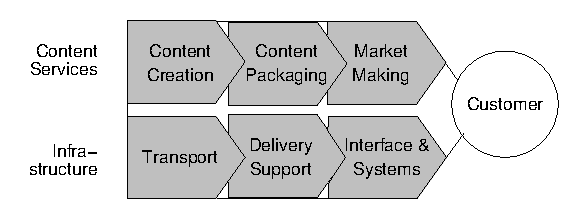
\includegraphics[width=0.4\textwidth]{indica_model}
%     \caption{INDICAn kaksitasoinen arvomalli.}
%     \label{fig:indica_model}
%   \end{center}
% \end{figure}

% Periaatteessa samaan kelluvaan objektiin voi laittaa useammankin kuvan
% (kuva~\ref{fig:tuplat}) tai asetella niitä taulukoilla.
% Jos tarvitset useita kuvia rinnakkain, harkitse
% myös pakettia \verb!subfigure!. Kuvien olisi hyvä olla samankokoisia.

% \begin{figure}[htb]
%   \begin{center}
%     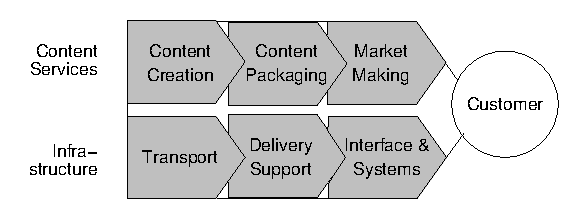
\includegraphics[height=20mm]{indica_model}
%     %\hfill  % toinen vas. reunaan, toinen oikeaan
%     \hspace{10mm}  % sentti väliä kuville
%     
\includegraphics[height=20mm]{AaltoSCI_FI_1}
%     \caption{Kaksi kuvaa rinnan esimerkkinä.}
%     \label{fig:tuplat}
%   \end{center}
% \end{figure}

% Yksinkertainen taulukko, joka ei ole kelluva ja siten sen pitäisi
% latoutua heti tämän tekstin alle. Tässä komento \verb!\topcaption!
% kyllä varaa itselleen ``Taulukko 1'', mutta tekstiä ei näy missään.

% \topcaption{Yksinkertainen taulukko}
% %\begin{center}                         % keskitys?
% \begin{tabular}{|l|l|l|} 
% \hline
% Tässä & sarakkeet & ei ole eroteltu mitenkään \\
% ja    & ne        & saattavat valua yli laidankin ikävästi \\
% \hline
% \end{tabular}
% %\end{center}

% Toinen kelluva perustaulukko, viitataan nyt taulukkoon~\ref{table:perustaulu}.
% Lähdetekstiä lukiessa näet tilde-merkin, joka pakottaa välilyönnin
% mutta estää rivinvaihdon.

% \begin{table}[ht]
% \caption{Tässä perustaulukko.}
% \label{table:perustaulu}
% \begin{center}
% \begin{tabular}{|l|l|l|} 
% \hline
% Tässä & sarakkeet & ei ole eroteltu mitenkään \\
% \hline
% ja    & ne        & saattavat valua yli laidankin ikävästi, %
%                    siksi käytä taulukkoa~\ref{table:dvbt_param}. %
%                    Teksti katoaa jonnekin sivun ulkopuolelle. \\
% \hline
% Nro   & Nro       & Nro \\
% \hline
% $-4$  & $8$       & $12$ \\
% \hline
% \end{tabular}
% \end{center}
% \end{table}

% Vielä kolmas esimerkki taulukosta, jossa sarakkeiden leveys määritelty
% ja soluissa voi olla useampi rivi tekstiä. Katso
% taulukko~\ref{table:dvbt_param}.

% \begin{table}[th]
% \caption{The DVB-T transmission parameters.}
% \label{table:dvbt_param}
% \begin{center}
% \begin{tabular}{|p{0.35\textwidth}|p{0.45\textwidth}|} 
%     \hline
% Parameter & Typical values \\
%     \hline
%     \hline
% Physical channel&8 MHz (also 6 MHz or 7 MHz possible)\\ 
%     \hline
% COFDM mode (number of subcarriers, 
% subcarrier width, 
% signal element length)
% &8k (6817, 1116 Hz, 896 $\mu$s) or 
% 2k (1705,4464 Hz, 224 $\mu$s)\\
%     \hline
% Guard interval (8k/4k duration)
% &1/4 (224/56 $\mu$s), 1/8 (112/28 $\mu$s),
%    1/16 (56/14 $\mu$s) or 1/32 (28/7 $\mu$s)\\
%     \hline
% Inner code rate &1/2, 2/3, 3/4, 5/6 or 7/8\\
%     \hline
% Signal  element constellation 
% &QPSK, 16-QAM or 64-QAM \\
%     \hline
% \end{tabular}
% \end{center}
% \end{table}


% Tässä esimerkki monisivuisesta taulukosta.
% EI toiminut aivat täydellisesti 27.1.2011: tablecaption hyppäsi edelliselle
% sivulle ennen ylläolevaa taulukkoa. Tämä supertabular taas ei voi olla 
% table-ympäristössä, kun muuten ei sivutu. supertabular on vain tabular,
% joka pitää kirjaa milloin sivun vaihto ja lisää automaatigisesti \end{tabular}
% ja uudestaa \begin{tabular}.
%\begin{center}
%\tablecaption{Esimerkki monisivuisesta taulukosta.}
%%\topcaption{taulukon nimi ylhäällä}
%%\bottomcaption{taulukon nimi alhaalla}
%\tablefirsthead{\hline \# & Sarakkeen aihe \\ \hline \hline }
%\tablehead{\hline \multicolumn{2}{|l|}{jatkoa edelliseltä sivulta} \\ %
%  \hline  \# & Sarakkeen aihe  \\ \hline \hline }
%\tabletail{\hline \multicolumn{2}{|r|}{jatkuu seuraavalle sivulle} \\ \hline}
%\tablelasttail{\hline}
%\label{table:pitkataulukko}
%\begin{supertabular}{|>{\bf}r|p{120mm}|} 
%\hline
%\multicolumn{2}{|l|}{Otsikko A} \\ 
%\hline
%1 & complex numbers, Carthesian and polar coordinate systems, Euler's formula   %\\
%2 & Euler's formula, cosine and sine, odd and even functions   \\
%3 & complex numbers, graphical notation   \\
%\hline 
%\multicolumn{2}{|l|}{Otsikko B} \\ 
%\hline
%14 & analog, discrete-time and digital signal   \\
%17 & analog, discrete-time and digital signal   \\
%16 & digital signals and spectra, spectogram \\
%17 & Fourier series, Fourier transforms: CTFT, DTFT, DFT \\
%18 & time-frequency-domain analysis and filtering \\
%21 & moving average (MA) filter, a simple FIR filter   \\
%22 & a simple IIR filter \\
%23 & flow / block diagram of a discrete-time system   \\
%24 & recognition of LTI systems, causal LTI systems, filter order, FIR, IIR   %\\
%25 & properties of LTI systems: linear, time-invariant, causal, stable   \\
%26 & shifted and scaled sequences in LTI system   \\
%31 & convolution as products of polynomials   \\
%32 & deconvolution   \\
%33 & parallel and cascade (series) LTI systems   \\
%34 & matched filter   \\
%35 & auto- and cross-correlation   \\
%37 & spectrum, CTFT, discrete-time Fourier transform (DTFT), %
% discrete Fourier transform (DFT)   \\
%38 & DTFT, computation from definition   \\
%39 & DTFT, using a transform table   \\
%40 & $2\pi$-periodic spectrum, DTFT   \\
%41 & magnitude/amplitude response, periodicity of DTFT   \\
%43 & sampling, Shannon's theorem   \\
%44 & impulse train and Fourier-series   \\
%45 & impulse train and sampling in frequency-domain   \\
%46 & sampling in frequency-domain   \\
%47 & aliasing   \\
%48 & sampling, aliasing, anti-aliasing   \\
%49 & anti-aliasing filter  \\
%51 & circular shift, DFT \\
%54 & amplitude response grafically from pole-zero-plot   \\
%55 & analysis of LTI IIR system, pole-zero plot   \\
%56 & transfer function, region of convergence (ROC)   \\
%57 & scaling factor   \\
%63 & direct form (DF) structures   \\
%70 & FIR-window method in digital filter design   \\
%71 & computational comparisons between IIR and FIR filters   \\
%73 & FFT computational complexity   \\
%74 & radix-2 DIT FFT algorithm   \\
%75 & binary addition and substraction, two's complement  \\
%78 & roundoff noise in FIR filters   \\
%79 & signal-to-noise ration (SNR) \\
%80 & error-feedback structure   \\
%81 & up- and downsampling in time- and frequency domain   \\
%82 & multirate system analysis   \\
%83 & linearity of up- and downsampling systems   \\
%84 & filter bank   \\
%85 & interpolated FIR filter (IFIR), FIR window method design  \\
%\end{supertabular}
%\end{center}


% \subsubsection{Matematiikka}
% \label{sec:esimmatematiikka}

% Lyhyet matemaattiset kaavat voi kirjoittaa tekstin
% sisään $E_{\textrm{total}} = m_i c^2$, mutta kaavat, joita käytetään, 
% kannattaa keskittää
% %
% \begin{equation}
% \label{eq:kaava1}
% x^2 + y^2 = 1 
% \end{equation}
% %
% josta lyhyempi versio ilman kaavan numerointia
% %
% \[ x^2 + y^2 = 1 \]
% %
% tai jakaa useammalle riville
% \begin{equation}
% \label{eq:kaava2}
% \begin{aligned}
% x^2 + y^2 &= 1 \\
%         x &= \sqrt{1-y^2}
% \end{aligned}
% \end{equation}
% %

% Kreikkalaiset kirjaimet löytyvät taulukosta~\ref{table:kreikka}.

% \begin{table}
% \caption{Kreikkalaiset kirjaimet}
% \label{table:kreikka}
% \begin{center}
% \begin{tabular}{|llllllll|}
% \hline
% $\alpha$        &$\theta$       &o              &$\tau$         &%
% $\beta$         &$\vartheta$    &$\pi$          &$\upsilon$     \\
% $\gamma$        &$\gamma$       &$\varpi$       &$\phi$         &%
% $\delta$        &$\kappa$       &$\rho$         &$\varphi$      \\
% $\epsilon$      &$\lambda$      &$\varrho$      &$\chi$         &%
% $\varepsilon$   &$\mu$          &$\sigma$       &$\psi$         \\
% $\zeta$         &$\nu$          &$\varsigma$    &$\omega$       &%
% $\eta$          &$\xi$          &               &               \\
% \hline
% $\Gamma$        &$\Lambda$      &$\Sigma$       &$\Psi$         &%
% $\Delta$        &$\Xi$          &$\Upsilon$     &$\Omega$       \\
% $\Theta$        &$\Pi$          &$\Phi$         & & & & &       \\
% \hline
% \end{tabular}
% \end{center}
% \end{table}

% Matematiikkaan liittyviä ohjeistusta löytyy esim. \citet{lyhyt2e}.
% Makroja sisältävästä tiedostosta \verb!makroja.tex! löytyy joitakin
% esimerkkejä, kuten 
% %
% \[ \myInt{-\infty}{0}{e^{x}}{x} \]
% %

% \subsubsection{Algoritmit ja ohjelmalistaukset}

% Työlle oleellisen tulostuslistauksen voi laittaa
% \verb!verbatim!-ympäristöön.
% %
% \begin{verbatim}
% Output written on main.pdf (23 pages, 268760 bytes).
% Transcript written on main.log.
% \end{verbatim}
% %
% \begin{sloppypar}
% Algoritmien ja pseudokoodin esittämiseen tarvitaan esimerkiksi
% \verb!algorithmic!- ja \verb!algorithm!-paketit.  Ohjelman esittelyn
% voi tehdä vaikkapa \verb!program!-paketin avulla.  Ohjelmakoodia ei
% tyypillisesti lisätä edes liitteeksi.  Jos näin kuitenkin tehdään,
% käytä ylläolevia tai esimerkiksi \verb!listinginput!-komentoa. Näiden
% käyttöön löytyy apua Internetistä.
% % Katso esim. http://en.wikibooks.org/wiki/LaTeX/Algorithms_and_Pseudocode
% \end{sloppypar}

% \subsection{Viittaukset ja lähdeluettelo}
% \label{sec:esimviitteet}


% \subsubsection{Ristiinviittaukset}
% \label{sec:esimristiviite}

% Ristiinviittauksia taulukkoon, kuvaan, kappaleeseen tai muuhun voi
% tehdä \verb!\ref!-komennolla, kuten tässä
% kuvaan~\ref{fig:indica_model}.  Isossa työssä voi olla näppärä antaa
% selailun nopeuttamiseksi myös sivunumero: kuva~\ref{fig:indica_model}
% löytyy sivulta~\pageref{fig:indica_model}. Tilde-merkki pakottaa
% välin, mutta sitoo sen niin, etteivät ne esiinny eri riveillä.

% Johdantoluvun lopussa tyypillisesti esitellään kirjan rakenne, joten
% voi viitata, että luvussa~\ref{sec:esimluettelo} tarkastellaan sitä ja
% tätä, luvussa~\ref{sec:esimtekstiviite} tuotakin. Englanniksi
% kirjoitettaessa isolla etukirjaimella ``Figure~\ref{fig:indica_model} on
% page~\pageref{fig:indica_model}'' ja ``Section~\ref{sec:esimtekstiviite}''.





% kokeillaan vähän vapaampaa, kun natbibiin kohdalla rivivaihto
% \begin{sloppypar}
% Katso eri tapoja tekstiviitteiden muotoiluun sivulta
% \url{http://merkel.zoneo.net/Latex/natbib.php}.
% Viittauskomennot  \verb!\citet! ja \verb!\citep! ovat
% hyviä tekijä-vuosi-tavassa \verb!natbib!iin liittyen
% ja \verb!\cite! on perusviittauskomento.
% \end{sloppypar}

% Pari esimerkkiä:
% % \citet
% \citet[s. 21]{Teekkari2010} on havainnut asian jos toisenkin. 
% % \citep
% Tämä ja tuo uusi havainto on vahvistanut teoriaa~\citep[s. 22]{Teekkari2010}.
% % \citep
% Joku asia on selitetty tarkasti monissa lähteissä 
% \citep[katso][s. 27]{Teekkari2010}.
% % KATSO LISÄÄ: http://merkel.zoneo.net/Latex/natbib.php

% \verb!tktl!-tyylin lähdetiedostoa \verb!tktl.dtx! ei ole
% muokattu Aalto-yliopiston käyttöön, joten esimerkiksi 
% lähdeviitteen merkintätyyppi \verb!@MasterThesis! tuottaa lähdeluetteloon
% tekstin ``Pro gradu'' (kts. \verb!finnbst.tex!).
% Tämä voidaan muuttaa antamalla kyseisen merkintätyypin kentälle
% \verb!type! arvo ``Diplomityö''. 

% \subsubsection{Lähdeluettelo}
% \label{sec:esimlahdeluettelo}

% Lähdeluettelon tulisi nyt ilmaantua dokumentin loppuun
% automaattisesti. Jos sitä ei näy ja etenkin jos tekstiviitteiden
% paikalla on kysymysmerkkejä, niin muista ajaa \verb!bibtex main!.

% --------------------------------------------------------------------

% Tätä käytetään vain testaustarkoituksiin, kun halutaan katsoa 
% miten sivu täyttyy pelkästä tekstistä tai miten fonttikoko
% vaikuttaa. 
%


% --------------------------------------------------------------------

\section{Conclusion}

% Loppuluku päättää työn. Luvun nimi on tyypillisesti ``yhteenveto'' tai
% ``johtopäätöksiä''. Valitse se otsikko, joka tuntuu sopivammalta työsi
% luonteeseen. Joka tapauksessa loppuluku sisältää niin työn yhteenvedon
% kuin johtopäätöksiä työn tulosten perusteella. Pääajatus on antaa
% lukijalle selvä kuva siitä, miten johdannossa asetettuihin
% tavoitteisiin työssä vastattiin.

% Käsittele loppupuvussa seuraavia asioita (jotakuinkin tässä järjestyksessä):
% %
% \begin{itemize}
%   \item Muistutus työn tavoitteista (sidoksisuus johdantoon)
%   \item Päätulokset kootaan yhteen, pohditaan niiden merkitystä
%   \item Suositukset konkreettisiksi toimenpiteiksi (``Mitä sitten?'' 
% Nyt kun käytössä on tämän työn myötä tullut tieto, 
% mitä se nyt tarkoittaa tälle asialle/alalle.)
%   \item Tulosten soveltuvuus, käyttöön liittyvät rajoitukset
%   \item Jatkotutkimustarve 
% (``Tulevaisuudessa olisi mielenkiintoista selvittää...'' tms.)
%   \item Työn onnistumisen arviointi 
% (Huom! Älä arvioi omaa kirjoitusprosessiasi vaan tekemääsi tutkimusta)
% \end{itemize}

% --------------------------------------------------------------------

